\subsection{集中型再グループ化}
バッテリー残量の平準化のため,センサノードのグループ再構成\ref{fig:group_reconstruction_concentrately}を行う.NSはGLから取得したデータ(センサデータ・信号強度・バッテリー残量等)を用いて最適なグループを再構成する.展開時にシードノードが作成した到達性リストにあるノード重複情報を用いたグループ間でのノード移動やGLの交代などの組み合わせを検討する.これにより,センサネットワーク全体の消費電力を平準化でき,センサ交換機会の削減が見込める.

\begin{figure}[]
    \begin{center}
    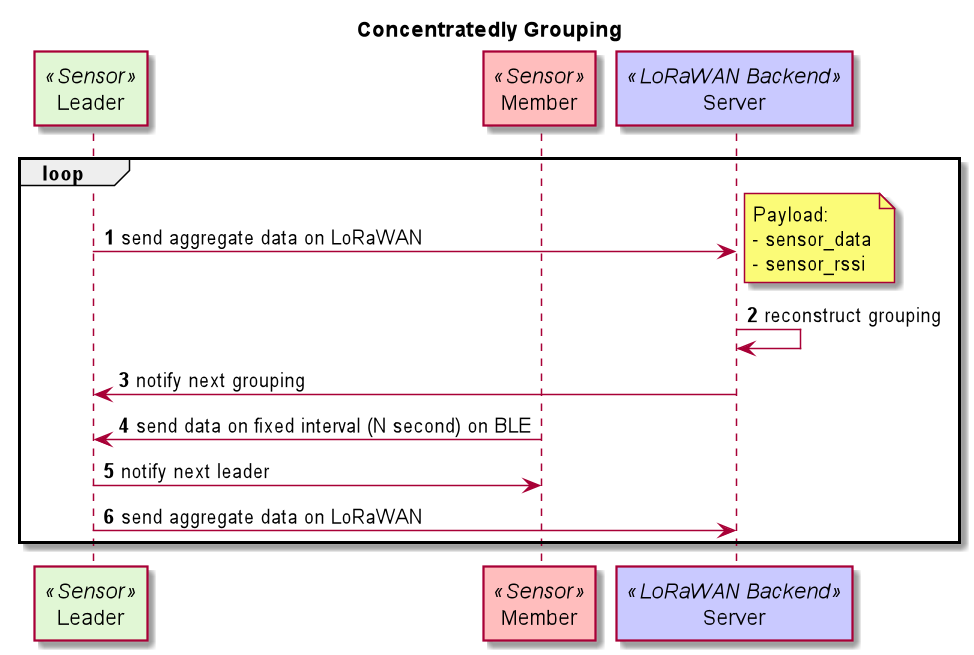
\includegraphics[width=14cm]{figures/グループ化_集中的.png}
    \caption{集中型グループ化}
    \label{fig:group_reconstruction_concentrately}
    \end{center}
\end{figure}